%\VignetteEngine{knitr::knitr}
%\VignetteIndexEntry{Grade of Membership Clustering and Visualization using CountClust}
%\VignettePackage{CountClust}

% To compile this document
% library('knitr'); rm(list=ls()); knit('CountClust/vignettes/count-clust.Rnw')
% library('knitr'); rm(list=ls()); knit2pdf('CountClust/vignettes/count-clust.Rnw'); openPDF('count-clust.pdf')
% !Rnw weave = knitr

\documentclass[12pt]{article}\usepackage[]{graphicx}\usepackage[usenames,dvipsnames]{color}
%% maxwidth is the original width if it is less than linewidth
%% otherwise use linewidth (to make sure the graphics do not exceed the margin)
\makeatletter
\def\maxwidth{ %
  \ifdim\Gin@nat@width>\linewidth
    \linewidth
  \else
    \Gin@nat@width
  \fi
}
\makeatother

\definecolor{fgcolor}{rgb}{0.345, 0.345, 0.345}
\newcommand{\hlnum}[1]{\textcolor[rgb]{0.686,0.059,0.569}{#1}}%
\newcommand{\hlstr}[1]{\textcolor[rgb]{0.192,0.494,0.8}{#1}}%
\newcommand{\hlcom}[1]{\textcolor[rgb]{0.678,0.584,0.686}{\textit{#1}}}%
\newcommand{\hlopt}[1]{\textcolor[rgb]{0,0,0}{#1}}%
\newcommand{\hlstd}[1]{\textcolor[rgb]{0.345,0.345,0.345}{#1}}%
\newcommand{\hlkwa}[1]{\textcolor[rgb]{0.161,0.373,0.58}{\textbf{#1}}}%
\newcommand{\hlkwb}[1]{\textcolor[rgb]{0.69,0.353,0.396}{#1}}%
\newcommand{\hlkwc}[1]{\textcolor[rgb]{0.333,0.667,0.333}{#1}}%
\newcommand{\hlkwd}[1]{\textcolor[rgb]{0.737,0.353,0.396}{\textbf{#1}}}%
\let\hlipl\hlkwb

\usepackage{framed}
\makeatletter
\newenvironment{kframe}{%
 \def\at@end@of@kframe{}%
 \ifinner\ifhmode%
  \def\at@end@of@kframe{\end{minipage}}%
  \begin{minipage}{\columnwidth}%
 \fi\fi%
 \def\FrameCommand##1{\hskip\@totalleftmargin \hskip-\fboxsep
 \colorbox{shadecolor}{##1}\hskip-\fboxsep
     % There is no \\@totalrightmargin, so:
     \hskip-\linewidth \hskip-\@totalleftmargin \hskip\columnwidth}%
 \MakeFramed {\advance\hsize-\width
   \@totalleftmargin\z@ \linewidth\hsize
   \@setminipage}}%
 {\par\unskip\endMakeFramed%
 \at@end@of@kframe}
\makeatother

\definecolor{shadecolor}{rgb}{.97, .97, .97}
\definecolor{messagecolor}{rgb}{0, 0, 0}
\definecolor{warningcolor}{rgb}{1, 0, 1}
\definecolor{errorcolor}{rgb}{1, 0, 0}
\newenvironment{knitrout}{}{} % an empty environment to be redefined in TeX

\usepackage{alltt}

\newcommand{\ecostructure}{\textit{ecostructure}}
\usepackage{dsfont}
\usepackage{cite}




\RequirePackage{/Library/Frameworks/R.framework/Versions/3.3/Resources/library/BiocStyle/resources/tex/Bioconductor}

\AtBeginDocument{\bibliographystyle{/Library/Frameworks/R.framework/Versions/3.3/Resources/library/BiocStyle/resources/tex/unsrturl}}



\bioctitle[\ecostructure{} - Grade of Membership Model and Visualization for ecological species abundance data]{\ecostructure{} - Grade of Membership Model and Visualization for ecological species abundance data}
\IfFileExists{upquote.sty}{\usepackage{upquote}}{}
\begin{document}

\maketitle

\section{Introduction}

The \textbf{ecostructure} R package is primarily aimed at providing tools and functions to replicate the statistical analysis in this paper. However we note that its toolbox is generic enough in handling and analyzing other species abundance data. We provide the bird species abundance data along with the relevant sample metadata and species metadata as an ExpressionSet object in this package. We provide a pipeline for reading and processing the data and the metadata and also to extract or process the data corresponding to different axes of diversity - for example, phylogenetic, regional and trait-based. We discuss how the Grade of Membership (GoM) model can be fitted to the counts data and the results from the fit can be viewed using the Block Structure Plot representation, which is analogous to the STRUCTURE plot visualization in \cite{Rosenberg2002} \cite{Pritchard2000}, but can account for ordering and blocking metadata. This package is an upgraded version of the CountClust Bioconductor package due to Dey et al \cite{Dey2016} that is better suited at processing and analyzing the structure of ecological abundance data.

\section{Installation}

The \textbf{ecostructure} package is available on Github and can be installed as follows



\begin{knitrout}
\definecolor{shadecolor}{rgb}{0.969, 0.969, 0.969}\color{fgcolor}\begin{kframe}
\begin{alltt}
\hlkwd{library}\hlstd{(devtools)}
\hlkwd{install_github}\hlstd{(}\hlstr{"kkdey/ecostructure"}\hlstd{)}
\end{alltt}
\end{kframe}
\end{knitrout}

Load the package as

\begin{knitrout}
\definecolor{shadecolor}{rgb}{0.969, 0.969, 0.969}\color{fgcolor}\begin{kframe}
\begin{alltt}
\hlkwd{library}\hlstd{(ecostructure)}
\hlkwd{library}\hlstd{(Biobase)}
\end{alltt}
\end{kframe}
\end{knitrout}

For fitting the Grade of Membership model, we recommend the user to install the latest version of the \textbf{maptpx} package as follows.

\begin{knitrout}
\definecolor{shadecolor}{rgb}{0.969, 0.969, 0.969}\color{fgcolor}\begin{kframe}
\begin{alltt}
\hlkwd{library}\hlstd{(devtools)}
\hlkwd{install_github}\hlstd{(}\hlstr{"Taddylab/maptpx"}\hlstd{)}
\end{alltt}
\end{kframe}
\end{knitrout}


\section{Data Processing}

The bird taxonomic abundance data for 304 bird species across 38 Himalayan forest patches, together with the grid metadata and species metadata, are saved as an ExpressionSet object which the user can read into R as follows.

\begin{knitrout}
\definecolor{shadecolor}{rgb}{0.969, 0.969, 0.969}\color{fgcolor}\begin{kframe}
\begin{alltt}
\hlstd{data} \hlkwb{<-} \hlkwd{get}\hlstd{(}\hlkwd{load}\hlstd{(}\hlkwd{system.file}\hlstd{(}\hlstr{"extdata"}\hlstd{,} \hlstr{"HimalayanBirdsData.rda"}\hlstd{,}
                             \hlkwc{package} \hlstd{=} \hlstr{"ecostructure"}\hlstd{)))}
\hlstd{taxonomic_counts} \hlkwb{<-} \hlkwd{t}\hlstd{(}\hlkwd{exprs}\hlstd{(data))}
\hlstd{taxonomic_counts[}\hlnum{1}\hlopt{:}\hlnum{5}\hlstd{,}\hlnum{1}\hlopt{:}\hlnum{5}\hlstd{]}
\end{alltt}
\begin{verbatim}
##    Macropygia_unchall Streptopelia_chinensis Streptopelia_senegalensis
## A2                  0                      0                         0
## A3                  0                      0                         0
## A4                  0                      0                         0
## A6                  0                      0                         0
## A7                  0                      0                         0
##    Columba_pulchricollis Streptopelia_orientalis
## A2                     0                       0
## A3                     0                       0
## A4                     0                       0
## A6                     0                       0
## A7                     2                       0
\end{verbatim}
\end{kframe}
\end{knitrout}


The corresponding grid metadata, comprising of the elevation, latitude and longitude information of the forest patches or grids, can be read as follows

\begin{knitrout}
\definecolor{shadecolor}{rgb}{0.969, 0.969, 0.969}\color{fgcolor}\begin{kframe}
\begin{alltt}
\hlstd{grid_metadata} \hlkwb{<-} \hlkwd{pData}\hlstd{(}\hlkwd{phenoData}\hlstd{(data))}
\hlkwd{head}\hlstd{(grid_metadata)}
\end{alltt}
\begin{verbatim}
##    Elevation North East WorE
## A2       198  27.0 92.9    E
## A3       734  27.0 92.4    E
## A4      1243  27.0 92.4    E
## A6      2629  27.1 92.5    E
## A7      2340  27.1 92.4    E
## A8       300  27.0 93.0    E
\end{verbatim}
\end{kframe}
\end{knitrout}

Finally, the species metadata, comprising of the bill traits, wing size, tarsus and mass of the birds, can be read as follows

\begin{knitrout}
\definecolor{shadecolor}{rgb}{0.969, 0.969, 0.969}\color{fgcolor}\begin{kframe}
\begin{alltt}
\hlstd{species_metadata} \hlkwb{<-} \hlkwd{pData}\hlstd{(}\hlkwd{featureData}\hlstd{(data))}
\hlkwd{head}\hlstd{(species_metadata)}
\end{alltt}
\begin{verbatim}
##                           bill_length bill_width bill_depth wing tarsus  mass
## Macropygia_unchall              11.08       4.26       4.97  198   26.3 168.0
## Streptopelia_chinensis          10.77       3.50       3.87  140   22.6 159.0
## Streptopelia_senegalensis        9.23       2.88       3.27  130   20.4  83.9
## Columba_pulchricollis           12.98       5.59       5.68  203   25.4 330.0
## Streptopelia_orientalis         10.88       4.09       3.90  192   25.5 233.0
## Chalcophaps_indica              11.77       3.61       4.42  151   26.3 121.0
\end{verbatim}
\end{kframe}
\end{knitrout}


Besides with the taxonomic data and metadata, we provide the phylogenetic tree data for the bird species as a \textit{.tre} file that can be loaded as follows, using the package \textbf{ape}.

\begin{knitrout}
\definecolor{shadecolor}{rgb}{0.969, 0.969, 0.969}\color{fgcolor}\begin{kframe}
\begin{alltt}
\hlstd{phylo_tree} \hlkwb{<-} \hlstd{ape}\hlopt{::}\hlkwd{read.tree}\hlstd{(}\hlkwd{system.file}\hlstd{(}\hlstr{"extdata"}\hlstd{,} \hlstr{"AllHim_Mar_27_2015.tre"}\hlstd{,}
                             \hlkwc{package} \hlstd{=} \hlstr{"ecostructure"}\hlstd{))}
\end{alltt}
\end{kframe}
\end{knitrout}


We also provide the shapefiles for the regional motif analysis.

\begin{knitrout}
\definecolor{shadecolor}{rgb}{0.969, 0.969, 0.969}\color{fgcolor}\begin{kframe}
\begin{alltt}
\hlstd{shp_file} \hlkwb{<-} \hlstd{ape}\hlopt{::}\hlkwd{read.tree}\hlstd{(}\hlkwd{system.file}\hlstd{(}\hlstr{"extdata"}\hlstd{,} \hlstr{"AllHim_Mar_27_2015.tre"}\hlstd{,}
                             \hlkwc{package} \hlstd{=} \hlstr{"ecostructure"}\hlstd{))}
\end{alltt}
\end{kframe}
\end{knitrout}

\section{Grade of Membership Model and Visualization}

Here we illustrate how one can fit the Grade of Membership model on the taxonomic data processed above and perform the visualization of the model fit using the Block Structure plot. Here we perform the fit for a number of clusters varying from 2 to 4.

\begin{knitrout}
\definecolor{shadecolor}{rgb}{0.969, 0.969, 0.969}\color{fgcolor}\begin{kframe}
\begin{alltt}
\hlstd{elevation_metadata}\hlkwb{=}\hlstd{grid_metadata}\hlopt{$}\hlstd{Elevation;}
\hlstd{east_west_dir} \hlkwb{=} \hlstd{grid_metadata}\hlopt{$}\hlstd{WorE;}
\hlstd{gom_fit} \hlkwb{<-} \hlstd{CountClust}\hlopt{::}\hlkwd{FitGoM}\hlstd{(taxonomic_counts,} \hlkwc{K}\hlstd{=}\hlnum{2}\hlopt{:}\hlnum{4}\hlstd{,} \hlkwc{tol}\hlstd{=}\hlnum{0.1}\hlstd{)}
\end{alltt}
\begin{verbatim}
## 
## Estimating on a 38 document collection.
## Fit and Bayes Factor Estimation for K = 2
## log posterior increase: 2484.4, 40.8, 27.4, 0.4, 1.4, 0.6, 5.4, 14.7, done.
## log BF( 2 ) = 2181.05
## 
## Estimating on a 38 document collection.
## Fit and Bayes Factor Estimation for K = 3
## log posterior increase: 4236.5, 16.5, 10.9, 3.3, 3.7, 1.1, 9.7, 11.8, 17.9, 3.2, 0.5, done.
## log BF( 3 ) = 2569.1
## 
## Estimating on a 38 document collection.
## Fit and Bayes Factor Estimation for K = 4
## log posterior increase: 3864.6, 18, 13.8, 1, done.
## log BF( 4 ) = 2124.78
\end{verbatim}
\end{kframe}
\end{knitrout}


\begin{verb} gom_fit \end{verb} is a list of size 3, with each component representing the model fit for the cluster $k$, where k varies from 2 to 4. The two main components of the model fit are the cluster membership proportion matrix $\omega$, given by \begin{verb} gom_fit[[k]]$omega \end{verb} and the cluster motif matrix \begin{verb} gom_fit[[k]]$theta \end{verb}, which is a description of the cluster using species compositions. We illustrate the results for $K=2$.

\begin{knitrout}
\definecolor{shadecolor}{rgb}{0.969, 0.969, 0.969}\color{fgcolor}\begin{kframe}
\begin{alltt}
\hlcom{############ membership proportion matrix (omega)  #################}

\hlstd{omega} \hlkwb{<-} \hlstd{gom_fit[[}\hlnum{2}\hlstd{]]}\hlopt{$}\hlstd{omega}
\hlkwd{head}\hlstd{(omega)}
\end{alltt}
\begin{verbatim}
##         topic
## document        1        2        3
##       A2 7.97e-05 1.00e+00 1.04e-04
##       A3 7.87e-05 9.99e-01 6.92e-04
##       A4 1.60e-04 9.98e-01 1.88e-03
##       A6 4.36e-04 1.24e-04 9.99e-01
##       A7 3.26e-04 9.73e-05 1.00e+00
##       A8 1.39e-04 1.00e+00 9.36e-05
\end{verbatim}
\begin{alltt}
\hlkwd{rowSums}\hlstd{(omega)}
\end{alltt}
\begin{verbatim}
## A2 A3 A4 A6 A7 A8 B1 B2 B3 B4 B5 D1 D3 G1 J1 J2 J4 J5 J6 K1 K2 K4 K5 K6 L1 M1 
##  1  1  1  1  1  1  1  1  1  1  1  1  1  1  1  1  1  1  1  1  1  1  1  1  1  1 
## M2 M3 M4 N1 N2 N3 S1 U3 U4 MA U1 U2 
##  1  1  1  1  1  1  1  1  1  1  1  1
\end{verbatim}
\begin{alltt}
\hlcom{########### cluster motif matrix (theta)  ###################}

\hlstd{theta} \hlkwb{<-} \hlstd{gom_fit[[}\hlnum{2}\hlstd{]]}\hlopt{$}\hlstd{theta}
\hlkwd{head}\hlstd{(theta)}
\end{alltt}
\begin{verbatim}
##                            topic
## phrase                             1        2        3
##   Macropygia_unchall        7.08e-07 6.05e-07 2.50e-03
##   Streptopelia_chinensis    2.95e-06 7.71e-03 6.89e-07
##   Streptopelia_senegalensis 7.09e-07 3.30e-03 6.87e-07
##   Columba_pulchricollis     7.08e-07 6.05e-07 1.25e-03
##   Streptopelia_orientalis   1.25e-02 2.50e-03 8.47e-07
##   Chalcophaps_indica        7.09e-07 3.30e-03 6.88e-07
\end{verbatim}
\begin{alltt}
\hlkwd{colSums}\hlstd{(theta)}
\end{alltt}
\begin{verbatim}
## 1 2 3 
## 1 1 1
\end{verbatim}
\end{kframe}
\end{knitrout}

We visulize the cluster membership proportions matrix \begin{verb} omega \end{verb} using a Block Structure Plot representation. In this representation, we use one metadata for forming blocks (the East/West direction in the figure below) and in each block, the samples are arranged by a second metadata ( Elevation in the figure below).

\begin{knitrout}
\definecolor{shadecolor}{rgb}{0.969, 0.969, 0.969}\color{fgcolor}\begin{kframe}
\begin{alltt}
\hlkwd{BlockStructure}\hlstd{(omega,} \hlkwc{blocker_metadata} \hlstd{= east_west_dir,}
               \hlkwc{order_metadata} \hlstd{= elevation_metadata,}
               \hlkwc{yaxis_label} \hlstd{=} \hlstr{"Elevation"}\hlstd{,}
               \hlkwc{levels_decreasing} \hlstd{=} \hlnum{FALSE}\hlstd{)}
\end{alltt}
\end{kframe}
\end{knitrout}


\begin{figure}[htp]
\begin{center}
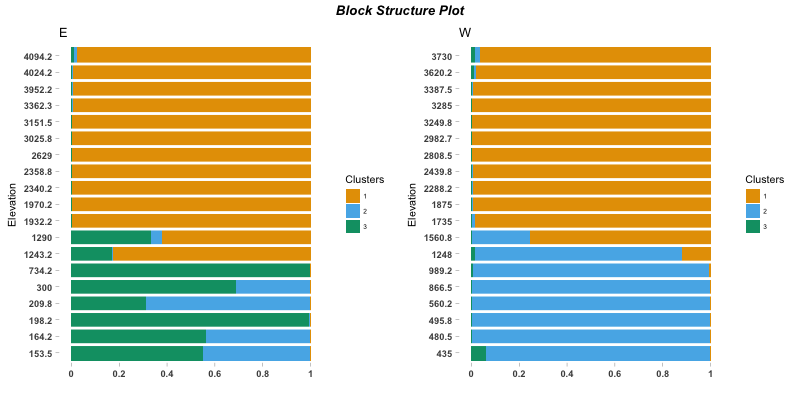
\includegraphics[width=6in,height=6in]{figure/block_structure.png}
\end{center}
\end{figure}

\newpage

\textbf{ecostructure} also provides tools to compare the GoM model fit for a particular $K$ (number of clusters) on the data, with respect to null model using the \begin{verb} nullmodel_GoM \end{verb} function. The package lets the user choose different null model types - \textit{frequency}, \textit{richness}, \textit{independent swap} and \textit{trial swap}.

\begin{knitrout}
\definecolor{shadecolor}{rgb}{0.969, 0.969, 0.969}\color{fgcolor}\begin{kframe}
\begin{alltt}
\hlkwd{nullmodel_GoM}\hlstd{(taxonomic_counts,} \hlkwc{K}\hlstd{=}\hlnum{2}\hlstd{,}
               \hlkwc{tol}\hlstd{=}\hlnum{500}\hlstd{,} \hlkwc{null.model}\hlstd{=}\hlstr{"frequency"}\hlstd{,}
               \hlkwc{iter_randomized}\hlstd{=}\hlnum{5}\hlstd{,} \hlkwc{plot}\hlstd{=}\hlnum{FALSE}\hlstd{)}
\end{alltt}
\begin{verbatim}
## 
## Estimating on a 38 document collection.
## Fit and Bayes Factor Estimation for K = 2
## log posterior increase: 2761, done.
## log BF( 2 ) = 334.73
## 
## Estimating on a 38 document collection.
## Fit and Bayes Factor Estimation for K = 2
## log posterior increase: 2889.8, done.
## log BF( 2 ) = 449.79
## 
## Estimating on a 38 document collection.
## Fit and Bayes Factor Estimation for K = 2
## log posterior increase: 2538.2, done.
## log BF( 2 ) = 298.7
## 
## Estimating on a 38 document collection.
## Fit and Bayes Factor Estimation for K = 2
## log posterior increase: 3015.5, done.
## log BF( 2 ) = 402.95
## 
## Estimating on a 38 document collection.
## Fit and Bayes Factor Estimation for K = 2
## log posterior increase: 2830.2, done.
## log BF( 2 ) = 350.39
## 
## Estimating on a 38 document collection.
## Fit and Bayes Factor Estimation for K = 2
## log posterior increase: 3003.6, done.
## log BF( 2 ) = 787.51
## $GoMBF.obs
## [1] 15725
## 
## $GoMBF.rand
## [1] 13621 13593 13229 12991 13387
## 
## $pval
## [1] 0
\end{verbatim}
\end{kframe}
\end{knitrout}

The function returns for a fixed $K$, the observed Bayes factor for the GoM model fit on the actual counts data, as well as the Bayes factor from applying GoM model on \begin{verb} iter_randomized \end{verb} many counts matrices generated under the specified null model. It also provdies a p-value of the observed Bayes factor with respect to the distribution of the Bayes factors from GoM on null model generated matrices.


\section{Processing data along different axes of diversity}

In this section, we demonstrate how \textbf{ecostructure} can be used to process
grid level counts data corresponding to different axes of diversity - regional, phylogenetic and trait-based. The idea is to obtain motifs or clusters defined by these different axes of diversity.

\subsection{Phylogenetic analysis}

For building the counts data based on phylogenetic diversity, we provide a function,\\
\begin{verb} collapse_counts_by_phylo () \end{verb} to collapse the taxa in the taxonomic counts data based on the phylogenetic similarity profile of the species.
The function reads in the taxonomic counts data and the phylogenetic tree data and a user defined cut off at which to slice the tree and collapse the taxa under each branch into a single phylogenetic unit.

\begin{knitrout}
\definecolor{shadecolor}{rgb}{0.969, 0.969, 0.969}\color{fgcolor}\begin{kframe}
\begin{alltt}
\hlstd{tree} \hlkwb{<-} \hlstd{ape}\hlopt{::}\hlkwd{read.tree}\hlstd{(}\hlkwd{system.file}\hlstd{(}\hlstr{"extdata"}\hlstd{,}
                                   \hlstr{"grids_tree_3_10_16.tre"}\hlstd{,}
                                    \hlkwc{package} \hlstd{=} \hlstr{"ecostructure"}\hlstd{))}
\hlstd{phylo_counts} \hlkwb{<-} \hlkwd{collapse_counts_by_phylo}\hlstd{(taxonomic_counts,}
                                         \hlstd{tree,} \hlkwc{collapse_at} \hlstd{=} \hlnum{10}\hlstd{)}
\hlkwd{dim}\hlstd{(phylo_counts)}
\end{alltt}
\begin{verbatim}
## [1]  38 196
\end{verbatim}
\end{kframe}
\end{knitrout}

We see that at the branching time \begin{verb} collapse_at \end{verb} of $10$, we get $196$ phylogenetic clusters of species, and the abundance data are summed over all taxa in a particular cluster to generate the output \begin{verb} phylo_counts \end{verb}.

We ue the data \begin{verb} phylo_counts \end{verb} as input for the \begin{verb} CountClust::FitGoM \end{verb} or  \begin{verb} CountClust::FitGoMpool \end{verb}  funtions to determine how clustering patterns are influenced by phylogenetic diversity.

\subsection{Regional analysis}

For the regional profile, \textbf{ecostructure} allows the user to create Global assemblage dispersion fields and build maps data from those fields. To create these assemblage dispersion fields, the user is required to obtain the shapefiles (\textit{.shp} files) for the all the species in the observed data.

One source of obtaining the \textit{.shp} files for mapping to geographic boundaries is from the Natural Earth webpage (www.naturalearthdata.com/downloads). For our Himalyan birds data, we obtained the \textit{.shp} files from BirdLife International (www.birdlife.org).

The user can put all the \textit{.shp} files in the \begin{verb} all_bird_shapefiles () \end{verb} and then, using this folder of shapefiles and the local taxonomic data, the user can create the global assemblage dispersion fields using the \begin{verb} CreateGlobalDispersionFields \end{verb} function as demonstrated below.

\begin{knitrout}
\definecolor{shadecolor}{rgb}{0.969, 0.969, 0.969}\color{fgcolor}\begin{kframe}
\begin{alltt}
\hlstd{disp} \hlkwb{<-} \hlkwd{CreateGlobalDispersionFields}\hlstd{(taxonomic_counts,}
              \hlkwc{shapefiles_dir} \hlstd{=} \hlstr{"all_bird_sjapefiles/"}\hlstd{)}
\end{alltt}
\end{kframe}
\end{knitrout}

We next show how the maps can be generated from the above dispersion field and the global shape file using the \begin{verb} CreateMapsFromDispersionFields \end{verb} function.

\begin{knitrout}
\definecolor{shadecolor}{rgb}{0.969, 0.969, 0.969}\color{fgcolor}\begin{kframe}
\begin{alltt}
\hlstd{dispersion.field} \hlkwb{<-} \hlkwd{readRDS}\hlstd{(}\hlkwd{system.file}\hlstd{(}\hlstr{"extdata"}\hlstd{,}
                    \hlstr{"dispersion_field_list.rds"}\hlstd{,} \hlkwc{package} \hlstd{=} \hlstr{"ecostructure"}\hlstd{))}
\hlstd{proj} \hlkwb{<-} \hlkwd{CRS}\hlstd{(}\hlstr{' +proj=longlat +ellps=WGS84'}\hlstd{)}
\hlstd{global_shapefile} \hlkwb{<-} \hlkwd{readShapeLines}\hlstd{(}\hlkwd{system.file}\hlstd{(}\hlstr{"extdata"}\hlstd{,}
         \hlstr{"ne_50m_admin_0_countries/ne_50m_admin_0_countries.shp"}\hlstd{,}
          \hlkwc{package} \hlstd{=} \hlstr{"ecostructure"}\hlstd{),} \hlkwc{proj4string}\hlstd{=proj)}
\hlkwd{par}\hlstd{(}\hlkwc{mfrow} \hlstd{=} \hlkwd{c}\hlstd{(}\hlnum{1}\hlstd{,}\hlnum{1}\hlstd{))}
\hlstd{maps} \hlkwb{<-} \hlkwd{CreateMapsFromDispersionFields}\hlstd{(dispersion.field, global_shapefile)}
\end{alltt}
\end{kframe}
\end{knitrout}

The function returns a list of map plots with as many elements as the number of sites. We demonstrate an example visualization of the map for the first site.

\begin{knitrout}
\definecolor{shadecolor}{rgb}{0.969, 0.969, 0.969}\color{fgcolor}\begin{kframe}
\begin{alltt}
\hlstd{maps[[}\hlnum{1}\hlstd{]]}
\end{alltt}
\end{kframe}
\end{knitrout}

\begin{figure}[htp]
\begin{center}
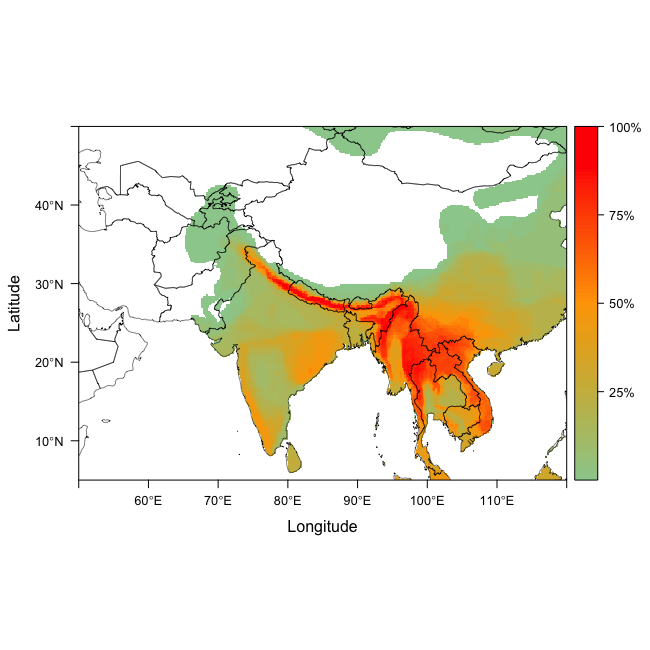
\includegraphics[width=6in,height=6in]{figure/maps.png}
\end{center}
\end{figure}

Finally, the user can generate the counts data corressponding to regional diversity profile using the \\
\begin{verb} DispersionFieldTocounts() \end{verb} function

\begin{knitrout}
\definecolor{shadecolor}{rgb}{0.969, 0.969, 0.969}\color{fgcolor}\begin{kframe}
\begin{alltt}
\hlstd{regional_counts} \hlkwb{<-} \hlkwd{DispersionFieldToCounts}\hlstd{(dispersion.field)}
\end{alltt}
\end{kframe}
\end{knitrout}

\begin{knitrout}
\definecolor{shadecolor}{rgb}{0.969, 0.969, 0.969}\color{fgcolor}\begin{kframe}
\begin{alltt}
\hlkwd{dim}\hlstd{(regional_counts)}
\end{alltt}
\begin{verbatim}
## [1]     38 201600
\end{verbatim}
\begin{alltt}
\hlstd{regional_counts[}\hlnum{1}\hlopt{:}\hlnum{5}\hlstd{,}\hlnum{1}\hlopt{:}\hlnum{5}\hlstd{]}
\end{alltt}
\begin{verbatim}
##    [,1] [,2] [,3] [,4] [,5]
## U1    0    0    0    0    0
## U2    1    1    1    1    1
## MA    0    0    0    0    0
## A2    0    0    0    0    0
## A3    0    0    0    0    0
\end{verbatim}
\end{kframe}
\end{knitrout}

The columns in this data represent 1 degree by 1 degree cells on which the dispersion fields are assembled. The cells are serially stacked along latitudes to form columns in the above matrix. This data is then used as an input for \begin{verb} CountClust::FitGoM \end{verb} or \begin{verb} CountClust::FitGoMpool \end{verb}  to determine how clustering patterns are influenced by regional diversity.


\subsection{Trait based analysis}

In order to build grid counts data based on functional diversity, we discuss two approaches.

In the first approach, we order the species based on some ordering metadata (like bill shape, size of the bird etc in our example). But there will be many zeros in the matrix as the species abundance data is sparse. To effectively account for the functional diversity and take into account the relatedness among the bird species, the zeros are filled in by kriging based on the species with non-zero abundance. We use the function \begin{verb} krige_counts \end{verb} to perform this.

\begin{knitrout}
\definecolor{shadecolor}{rgb}{0.969, 0.969, 0.969}\color{fgcolor}\begin{kframe}
\begin{alltt}
\hlstd{func_counts} \hlkwb{<-} \hlkwd{krige_counts}\hlstd{(taxonomic_counts,}
        \hlkwc{order} \hlstd{= species_metadata}\hlopt{$}\hlstd{bill_length,}
            \hlkwc{krige.control} \hlstd{=} \hlkwd{list}\hlstd{(}\hlkwc{cov.mod} \hlstd{=} \hlstr{"whitmat"}\hlstd{,} \hlkwc{sill}\hlstd{=}\hlnum{0.5}\hlstd{,} \hlkwc{smooth}\hlstd{=}\hlnum{.01}\hlstd{))}
\end{alltt}
\end{kframe}
\end{knitrout}

\begin{knitrout}
\definecolor{shadecolor}{rgb}{0.969, 0.969, 0.969}\color{fgcolor}\begin{kframe}
\begin{alltt}
\hlkwd{dim}\hlstd{(func_counts)}
\hlkwd{head}\hlstd{(func_counts[,}\hlnum{1}\hlopt{:}\hlnum{5}\hlstd{])}
\end{alltt}
\end{kframe}
\end{knitrout}


The other approach is to use a trait or traits  to collapse the bird species by performing hierarchical clustering of the bird species, cutting off a dendrogram at a particular level, thereby forming several clusters and then for each grid point, aggregating the counts data for all the species in the cluster. The cut level is chosen subjectively based on what proportion of variation in the actual abundance data is explained by the clusters at that level. We use the \begin{verb} trait_cluster() \end{verb} function in \textbf{ecostructure} to perform this, an application of which is demonstrated below.

\begin{knitrout}
\definecolor{shadecolor}{rgb}{0.969, 0.969, 0.969}\color{fgcolor}\begin{kframe}
\begin{alltt}
\hlstd{bill_traits} \hlkwb{<-} \hlkwd{as.matrix}\hlstd{(}\hlkwd{dist}\hlstd{(}\hlkwd{scale}\hlstd{(species_metadata[,}\hlkwd{c}\hlstd{(}\hlnum{1}\hlopt{:}\hlnum{3}\hlstd{)])))}
\hlstd{bill_trait_clust} \hlkwb{<-} \hlkwd{trait_cluster}\hlstd{(}\hlkwc{counts} \hlstd{= taxonomic_counts,}
                                  \hlkwc{traits} \hlstd{= bill_traits,} \hlkwc{prop_div}\hlstd{=}\hlnum{0.3}\hlstd{)}
\end{alltt}
\end{kframe}
\end{knitrout}

We first generate a traits matrix, with the columns representing the traits and rows corresponding to the species. Then we use that to perform a hierarchical clustering of species and cut the dendrogram at a specified level, given by  \begin{verb} prop_div \end{verb}.

The clusters of species formed by cutting the dendrogram are then used to collapse the counts data and reduce the original counts matrix with species along the columns to one with the clusters along the columns. This matrix can then used as input for the \begin{verb} CountClust::FitGoM \end{verb} or \begin{verb} CountClust::FitGoMpool \end{verb}  to determine how clustering patterns are influenced by species traits.

\section{Extras}

\textbf{ecostructure} provides additional functions for plotting a variable of interest (which could be the grades of membership or the motif pattern) against a metadata and a diversity measure or against two metadata in three way scatter plot functions.

An example of plotting a variable against two metadata are as follows.

\begin{knitrout}
\definecolor{shadecolor}{rgb}{0.969, 0.969, 0.969}\color{fgcolor}\begin{kframe}
\begin{alltt}
\hlstd{annotation} \hlkwb{=} \hlkwd{data.frame}\hlstd{(}\hlkwc{x_names} \hlstd{=} \hlkwd{c}\hlstd{(}\hlkwd{paste0}\hlstd{(}\hlstr{"A"}\hlstd{,}\hlnum{1}\hlopt{:}\hlnum{5}\hlstd{),} \hlkwd{paste0}\hlstd{(}\hlstr{"B"}\hlstd{,}\hlnum{1}\hlopt{:}\hlnum{5}\hlstd{)),}
\hlkwc{x} \hlstd{=} \hlkwd{c}\hlstd{(}\hlnum{0.5}\hlstd{,}\hlnum{2.0}\hlstd{,} \hlnum{3.2}\hlstd{,} \hlnum{4.6}\hlstd{,} \hlnum{6.3}\hlstd{,}  \hlnum{23.5}\hlstd{,} \hlnum{26.4}\hlstd{,} \hlnum{28.5}\hlstd{,} \hlnum{29.6}\hlstd{,} \hlnum{31.8}\hlstd{),}
\hlkwc{y1} \hlstd{=} \hlkwd{c}\hlstd{(}\hlnum{0.4}\hlstd{,} \hlnum{0.3}\hlstd{,} \hlnum{0.4}\hlstd{,} \hlnum{0.35}\hlstd{,} \hlnum{0.4}\hlstd{,} \hlnum{0.8}\hlstd{,} \hlnum{0.85}\hlstd{,} \hlnum{0.9}\hlstd{,} \hlnum{0.8}\hlstd{,} \hlnum{0.75}\hlstd{),}
\hlkwc{y2} \hlstd{=}\hlkwd{c}\hlstd{(}\hlnum{5}\hlstd{,} \hlnum{6.6}\hlstd{,} \hlnum{4}\hlstd{,} \hlnum{5.2}\hlstd{,} \hlnum{20}\hlstd{,} \hlnum{3.4}\hlstd{,} \hlnum{5.6}\hlstd{,} \hlnum{4.5}\hlstd{,} \hlnum{8}\hlstd{,} \hlnum{10}\hlstd{))}

\hlkwd{head}\hlstd{(annotation)}
\end{alltt}
\begin{verbatim}
##   x_names    x   y1   y2
## 1      A1  0.5 0.40  5.0
## 2      A2  2.0 0.30  6.6
## 3      A3  3.2 0.40  4.0
## 4      A4  4.6 0.35  5.2
## 5      A5  6.3 0.40 20.0
## 6      B1 23.5 0.80  3.4
\end{verbatim}
\begin{alltt}
\hlkwd{topic_meta_meta}\hlstd{(annotation)}
\end{alltt}
\end{kframe}
\end{knitrout}

\begin{figure}[htp]
\begin{center}
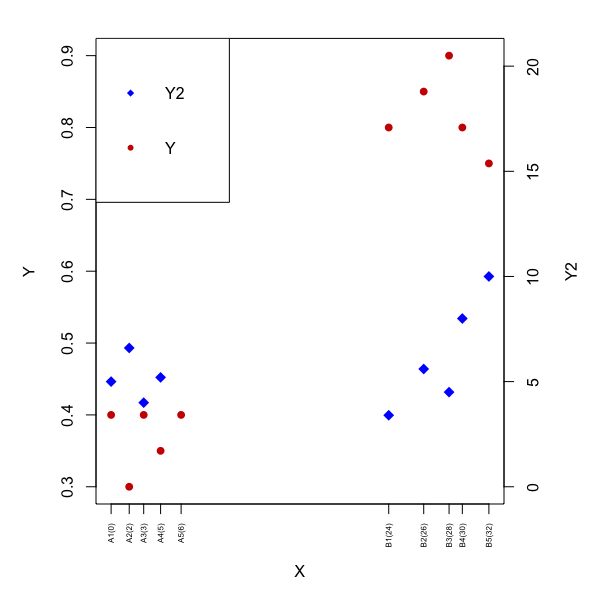
\includegraphics[width=6in,height=6in]{figure/topic_meta_meta.png}
\end{center}
\end{figure}


An example of plotting  a variable against two diversity measures as follows.

\begin{knitrout}
\definecolor{shadecolor}{rgb}{0.969, 0.969, 0.969}\color{fgcolor}\begin{kframe}
\begin{alltt}
\hlstd{annotation} \hlkwb{=} \hlkwd{data.frame}\hlstd{(}\hlkwc{x_names} \hlstd{=} \hlkwd{c}\hlstd{(}\hlkwd{paste0}\hlstd{(}\hlstr{"A"}\hlstd{,}\hlnum{1}\hlopt{:}\hlnum{5}\hlstd{),} \hlkwd{paste0}\hlstd{(}\hlstr{"B"}\hlstd{,}\hlnum{1}\hlopt{:}\hlnum{5}\hlstd{)),}
    \hlkwc{x} \hlstd{=} \hlkwd{c}\hlstd{(}\hlnum{0.5}\hlstd{,}\hlnum{2.0}\hlstd{,} \hlnum{3.2}\hlstd{,} \hlnum{4.6}\hlstd{,} \hlnum{6.3}\hlstd{,}  \hlnum{23.5}\hlstd{,} \hlnum{26.4}\hlstd{,} \hlnum{28.5}\hlstd{,} \hlnum{29.6}\hlstd{,} \hlnum{31.8}\hlstd{),}
    \hlkwc{y1} \hlstd{=} \hlkwd{c}\hlstd{(}\hlnum{0.4}\hlstd{,} \hlnum{0.3}\hlstd{,} \hlnum{0.4}\hlstd{,} \hlnum{0.35}\hlstd{,} \hlnum{0.4}\hlstd{,} \hlnum{0.8}\hlstd{,} \hlnum{0.85}\hlstd{,} \hlnum{0.9}\hlstd{,} \hlnum{0.8}\hlstd{,} \hlnum{0.75}\hlstd{),}
    \hlkwc{y2d} \hlstd{=}\hlkwd{c}\hlstd{(}\hlnum{5}\hlstd{,} \hlnum{6.6}\hlstd{,} \hlnum{4}\hlstd{,} \hlnum{5.2}\hlstd{,} \hlnum{20}\hlstd{,} \hlnum{3.4}\hlstd{,} \hlnum{5.6}\hlstd{,} \hlnum{4.5}\hlstd{,} \hlnum{8}\hlstd{,} \hlnum{10}\hlstd{))}

\hlkwd{head}\hlstd{(annotation)}
\end{alltt}
\begin{verbatim}
##   x_names    x   y1  y2d
## 1      A1  0.5 0.40  5.0
## 2      A2  2.0 0.30  6.6
## 3      A3  3.2 0.40  4.0
## 4      A4  4.6 0.35  5.2
## 5      A5  6.3 0.40 20.0
## 6      B1 23.5 0.80  3.4
\end{verbatim}
\begin{alltt}
\hlkwd{topic_meta_diversity}\hlstd{(annotation)}
\end{alltt}
\end{kframe}
\end{knitrout}

\begin{figure}[htp]
\begin{center}
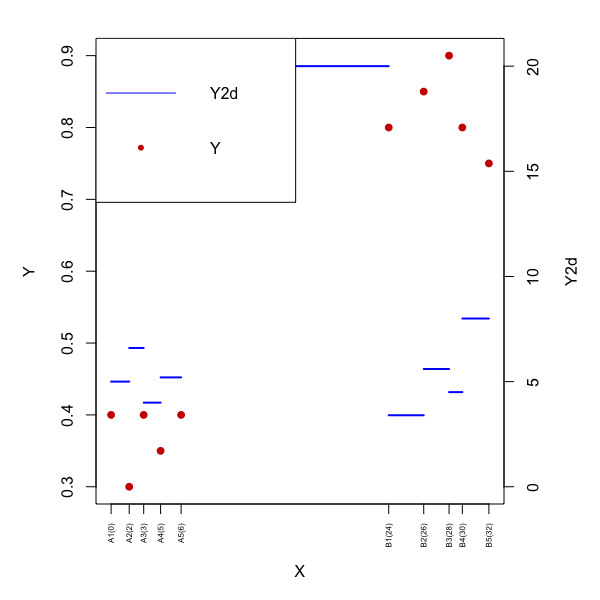
\includegraphics[width=6in,height=6in]{figure/topic-meta-diversity.png}
\end{center}
\end{figure}

\section{Session Info}

\begin{knitrout}
\definecolor{shadecolor}{rgb}{0.969, 0.969, 0.969}\color{fgcolor}\begin{kframe}
\begin{alltt}
\hlkwd{sessionInfo}\hlstd{()}
\end{alltt}
\begin{verbatim}
## R version 3.3.3 (2017-03-06)
## Platform: x86_64-apple-darwin13.4.0 (64-bit)
## Running under: macOS Sierra 10.12.5
## 
## locale:
## [1] en_US.UTF-8/en_US.UTF-8/en_US.UTF-8/C/en_US.UTF-8/en_US.UTF-8
## 
## attached base packages:
## [1] grid      parallel  stats     graphics  grDevices utils     datasets 
## [8] methods   base     
## 
## other attached packages:
##  [1] ecostructure_0.99.1   Biobase_2.34.0        BiocGenerics_0.20.0  
##  [4] maptools_0.9-2        SpatialExtremes_2.0-5 phytools_0.6-20      
##  [7] maps_3.2.0            ape_4.1               gridExtra_2.3        
## [10] rgdal_1.2-11          raster_2.5-8          sp_1.2-5             
## [13] ordtpx_0.0.1          slam_0.1-40           maptpx_1.9-3         
## [16] CountClust_0.1.2      ggplot2_2.2.1         knitr_1.16           
## 
## loaded via a namespace (and not attached):
##  [1] viridisLite_0.2.0       splines_3.3.3           gtools_3.5.0           
##  [4] expm_0.999-2            highr_0.6               stats4_3.3.3           
##  [7] latticeExtra_0.6-28     animation_2.5           numDeriv_2016.8-1      
## [10] lattice_0.20-34         limma_3.30.13           quadprog_1.5-5         
## [13] phangorn_2.2.0          digest_0.6.12           RColorBrewer_1.1-2     
## [16] colorspace_1.3-2        picante_1.6-2           cowplot_0.8.0          
## [19] Matrix_1.2-10           plyr_1.8.4              pkgconfig_2.0.1        
## [22] mvtnorm_1.0-6           scales_0.4.1            tibble_1.3.4           
## [25] combinat_0.0-8          mgcv_1.8-17             hexbin_1.27.1          
## [28] nnet_7.3-12             lazyeval_0.2.0          rasterVis_0.41         
## [31] mnormt_1.5-5            survival_2.40-1         magrittr_1.5           
## [34] evaluate_0.10           msm_1.6.4               nlme_3.1-131           
## [37] MASS_7.3-45             foreign_0.8-67          vegan_2.4-3            
## [40] tools_3.3.3             BiocStyle_2.2.1         stringr_1.2.0          
## [43] munsell_0.4.3           cluster_2.0.5           plotrix_3.6-6          
## [46] clusterGeneration_1.3.4 rlang_0.1.1.9000        igraph_1.1.1           
## [49] boot_1.3-18             gtable_0.2.0            flexmix_2.3-14         
## [52] reshape2_1.4.2.9000     zoo_1.8-0               fastmatch_1.1-0        
## [55] permute_0.9-4           modeltools_0.2-21       stringi_1.1.5          
## [58] SQUAREM_2016.8-2        Rcpp_0.12.12            scatterplot3d_0.3-40   
## [61] coda_0.19-1
\end{verbatim}
\end{kframe}
\end{knitrout}

\begin{thebibliography}

\bibitem{Dey2016}
Dey K, Hsiao J and Stephens M.
CountClust: Clustering and Visualizing RNA-Seq Expression Data using Grade of Membership Models. 2016.
\textit{R package version 0.1.2.} https://github.com/kkdey/CountClust

\bibitem{Pritchard2000}
Pritchard, Jonathan K., Matthew Stephens, and Peter Donnelly. 2000.
Inference of population structure using multilocus genotype data.
\textit{Genetics}. 155.2,  945-959.

\bibitem{Rosenberg2002}
Rosenberg NA, Pritchard JK,  Weber JL, Cann HM,  Kidd KK,  Zhivotovsky LA,  Feldman MW. 2002.
The genetic structure of human populations.
\textit{Science}. 298,  2381-2385.







\end{thebibliography}

\end{document}
